\chapter{Low Tech Microscopy} \index{Microscope! low tech}
\label{cha:microscopy}

\noindent Microscopes are powerful tools for teaching biology, and many of their benefits are hard to replace with local fabrications. However, simple materials can be used to achieve sufficient magnification to greatly expands students' understanding of the very small. They may view up close the anatomy of insects and even see cells.

\begin{multicols}{2}



\section{Water as a lens}
Water refracts light much the way glass does; a water drop with perfect curvature can make a powerful lens. A simple magnifier can be made by twisting a piece of wire around a nail and dipping the loop briefly into some water. Students can observe the optical properties of the trapped drop of water.

\section{Perfect circles}
Better imaging can be had if the drop is more perfect in shape -- the asymmetry of the wire twisting distorts the image. Search for a piece of thin but stiff plastic -- water bottles work well. Cut a small piece of this plastic, perhaps $1 \times 2$ centimeters. Near one end, make a hole, the more perfect the better. The best hole-cutting tool is a paper hole punch, available in many schools. With care, fine scissors or a pen knife will suffice; remove all burrs.
\begin{center}
%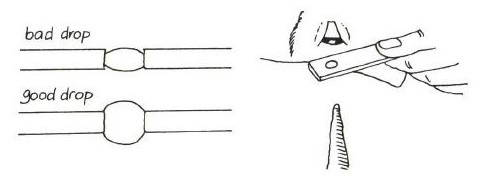
\includegraphics[width=8cm]{./img/vso/water-drop.jpg}
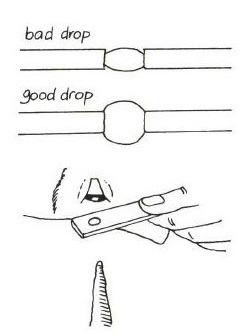
\includegraphics[width=0.4\textwidth]{./img/vso/water-drop-2.jpg}
\end{center}

\columnbreak

\section{Slides}
A slide and even cover slip may be made from the same plastic water bottles, although being hydrophobic they will not have the same properties of glass when making wet mounts. Improvise a method for securing the punctured plastic over the slide; ideally the vertical spacing can be closely adjusted to focus.
\begin{center}
%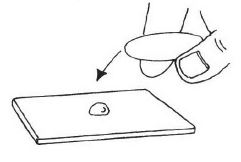
\includegraphics[width=4cm]{./img/vso/slide-cover-slip.jpg}
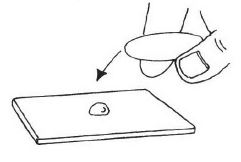
\includegraphics[width=0.45\textwidth]{./img/vso/slide-cover-slip.jpg}
\end{center}

\section{Backlighting}
On a bright day, there may not be any need for additional lighting, but in most classrooms the image will be too dim to be easily seen. The sun is a powerful light source, though not always convenient. Flashlights are generally inexpensive and available; many cell phones have one built in the end. To angle the light into the slide, find either a piece of mirror glass, wrinkle-free aluminum foil, the metalized side of a biscuit wrapper, etc.

Experiment with a variety of designs to see what works best given the materials available to your school. If you use a slide of onion cells stained with iodine solution
%(see \nameref{cha:sourcesofchemicals}, p.~\pageref{cha:sourcesofchemicals})
, your students should be able to see cell walls and nuclei.

\vfill
\columnbreak

\section[Simple Microscopes and Magnifiers]{Simple Microscopes and \hfill \\ Magnifiers}

\subsection{Clear-Container Magnifiers}
\begin{center}
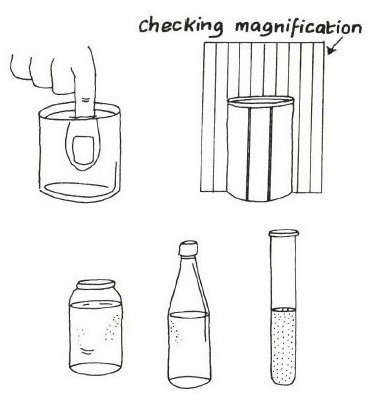
\includegraphics[width=0.4\textwidth]{./img/vso/container-microscope-2.jpg}
\end{center}

Any of these containers filled with water will make good magnifiers.

\subsection{Simple Microscope}
\begin{center}
%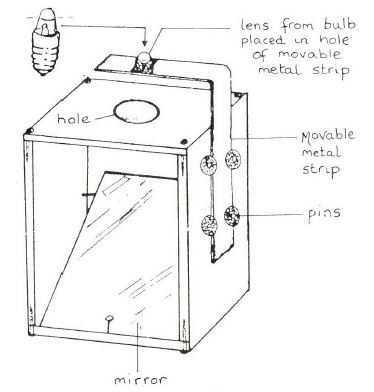
\includegraphics[width=0.49\textwidth]{./img/source/simple-microscope.jpg}
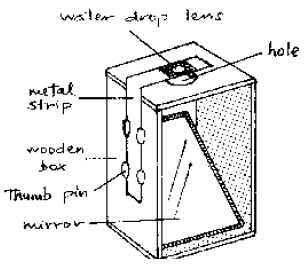
\includegraphics[width=0.49\textwidth]{./img/source/simple-microscope-2.png}
\end{center}

Construct a small wooden box from plywood as
shown (or use a small cardboard carton such as
a light bulb box). Make a round hole of 2 cm
diameter, at the top. Fit a small mirror (glass or
polished metal) in the box, angled to reflect light
up through the hole. Make a small hole (about 6
mm) in a strip of metal. Remove the round top
from a pen-torch bulb and secure it in the strip
using adhesive tape. Carefully cut off the tape
where it may cover the lens. Bend the strip, then
fix it to the side of the box, so that it can be
moved up and down. Drawing pins or nails
could be used for this. The object is focused by
moving this strip. Note the eye should be placed
as near as possible to the lens when viewing.

\vfill
\columnbreak

\subsection[Simple Compound Microscope]{Simple Compound \hfill \\ Microscope}
\begin{center}
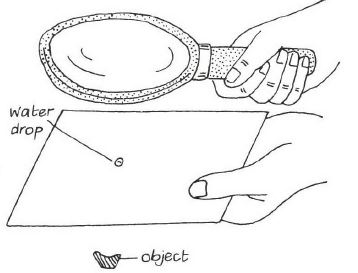
\includegraphics[width=0.4\textwidth]{./img/vso/compound-microscope.jpg}
\end{center}

\begin{itemize*}
\item Using 2 lenses together allows much greater magnification. 
\item Use a hand lens to make a water drop into a more powerful magnifier. 
\item Try using a hand lens with a lens from a torch bulb to make another simple compound microscope.
\end{itemize*}


\subsection{Card Bridge Microscope}
\begin{center}
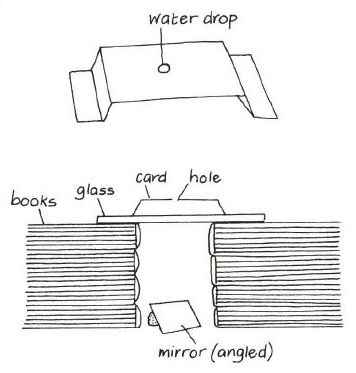
\includegraphics[width=0.4\textwidth]{./img/vso/card-microscope.jpg}
\end{center}

\begin{itemize*}
\item Place a water drop in the card `bridge'. 
\item Place this on a sheet of glass as shown. 
\item Place the object you are looking
at on the glass. This
arrangement is most suitable
for thin items, e.g. sections of leaves. 
\item Experiment with the angle of
the mirror so that light shines
up through the specimen.
\item Use this arrangement with a
hand lens to produce a
compound microscope.
\end{itemize*}

\vfill

\end{multicols}